%We document the retrieval, enhancement, labelling and augmentation of [the|our] data set [used for the experiments].
% We document how we retrieve, enhance, label and augment our data set.
We document the retrieval, enhancement and augmentation of our data set.

\subsection{Database}
We use the Breast Cancer Digital Repository (BCDR-DM) database, specifically, the BDCR-D01 data set, which is composed of patients with at least one breast mass.
%We curated it to delete patients with breast implants.
We select 256 digital mammograms from 63 patients.
A patient with breast implants (511) was ignored.
Mammograms are 8-bit grayscale images with 0.07mm spatial resolution sized $3328\times 4084$, $2816\times 3072$ or $2560 \times 3328$ pixels equivalent to $23.3 \times 28.6$, $19.7 \times 21.5$ and $17.9 \times 23.3$ centimeters.
%Each lesion's segmentation, type (mass, microcalcification, calcification, axillary adenopathy, architectural distortion or stroma distortion) and biopsy result (benign or malignant) are provided.
The data set provides the segmentation, type (mass, microcalcification, calcification, axillary adenopathy, architectural distortion or stroma distortion) and biopsy result (benign or malignant) of each lesion.
%Segmentation, type and biopsy result for each lesion are provided. 
%Each lesion is segmented and its type (mass, microcalcification, calcification, axillary adenopathy, architectural distortion or stroma distortion) and biopsy result (benign or malignant) are supplied.
We disregard patient data (age and breast density) and image features (intensity, texture, shape and location descriptors).
%do not make use of/employ/ ignore/disregard

We generate our labels using the provided lesion outlines and thresholding the mammogram to zero to separate the background.
%and separating the background by thresholding to zero. 
%Labels were generated using the provided outlines and thresholding the background to zero.
Masses (benign or malignant) appear as white; breast area as gray and background as black (Fig.~\ref{subfig:Preprocessinga}).

Digital mammograms have higher image quality and lack any marks or scanning artifacts present in digitized film mammograms; this allows the network to learn sharper features easying segmentation.
Although we only dispose of few mammograms, we overcome this problem by augmenting our data set and training on overlapping patches.

\subsection{Data division}
We divide patients in our data set into a training (75\%), validation (10\%) and test (15\%) set~(Tab.~\ref{tab:DataSetSummary}).

\begin{table}[h]
	\centering
	\begin{tabular}{lcccc}
		\hline
		&\textbf{Training} & \textbf{Validation} & \textbf{Test} & \textbf{Total}\\
		\hline 
		Percentage of data set	&75	&10	&15	&100\\
		Number of patients 	&47	&6	&10	&63\\
		Number of mammograms 	&196	&22	&38	&256\\
		Number of masses 	&104	&14	&21	&139\\
		Mammograms (after augmentation) &1568 &176 &38	&1782\\
		\hline
	\end{tabular}
	\caption[Data set summary]{Data set summary}
	\label{tab:DataSetSummary}
\end{table}

\subsection{Image enhancement}
We zero any pixel below the mean pixel intensity of the image (calculated only on the breast area) and scale the rest linearly to cover the entire intensity range (0-255); this reduces all small variations in the background to black and increases the contrast of the image (Fig.~\ref{subfig:Preprocessingb}).
%Background reduction reduces all small variations in the background to black and linear normalization increases the contrast of the remaining image. 

Background reduction plus contrast normalization highlights breast masses, which are brighter than normal breast tissue; normalizes images from patients with darker or lighter tissue and improves convergence~\cite{Arevalo2016}. However, it may destroy important texture information by blending it with the background or cause false positives by highlighting dense tissue.

\subsection{Resizing}
We resize our images to hold a $2 \times 2$ cm area into $112 \times 112$ pixels---roughly a 2.5 downsampling factor.
%We use Lanczos interpolation for mammograms and nearest neighbor interpolation for labels; both present in PILLOW, the Python Image Library.
We resize them with PILLOW, the Python Image Library, using Lanczos interpolation for mammograms and nearest neighbor interpolation for labels (Fig.~\ref{subfig:Preprocessingc}).

Our convolutional network has a $112 \times 112$ receptive field (spatial dimensions of the input volume).
We resize our images to contain $2 \times 2$ cms in this area considering that masses are rarely bigger than 2cm (length of the long axis)~\cite{Sahiner1996} and we want our network to see a good portion of the lesion during classification.
Lanczos interpolation is a high quality downsampling filter recommended by PILLOW and nearest neighbor interpolation assures that the reduced label contains only valid values (white, gray and black).


\subsection{Cropping}
We calculate the bounding box of the breast area in the label image and crop the mammogram and the label to delete unnecesary black spaces (Fig.~\ref{subfig:Preprocessingd}). 
Because our network produces segmentations downsampled by a factor of 16, we make sure the dimensions of the cropped image are multiples of 16 (cropping a slighlty bigger area if needed) so that the downsampling of the mammograms and upsampling of the produced segmentations are exact.

\begin{figure}[h]
	\centering
	\begin{subfigure}{4.2 cm}
		\centering
                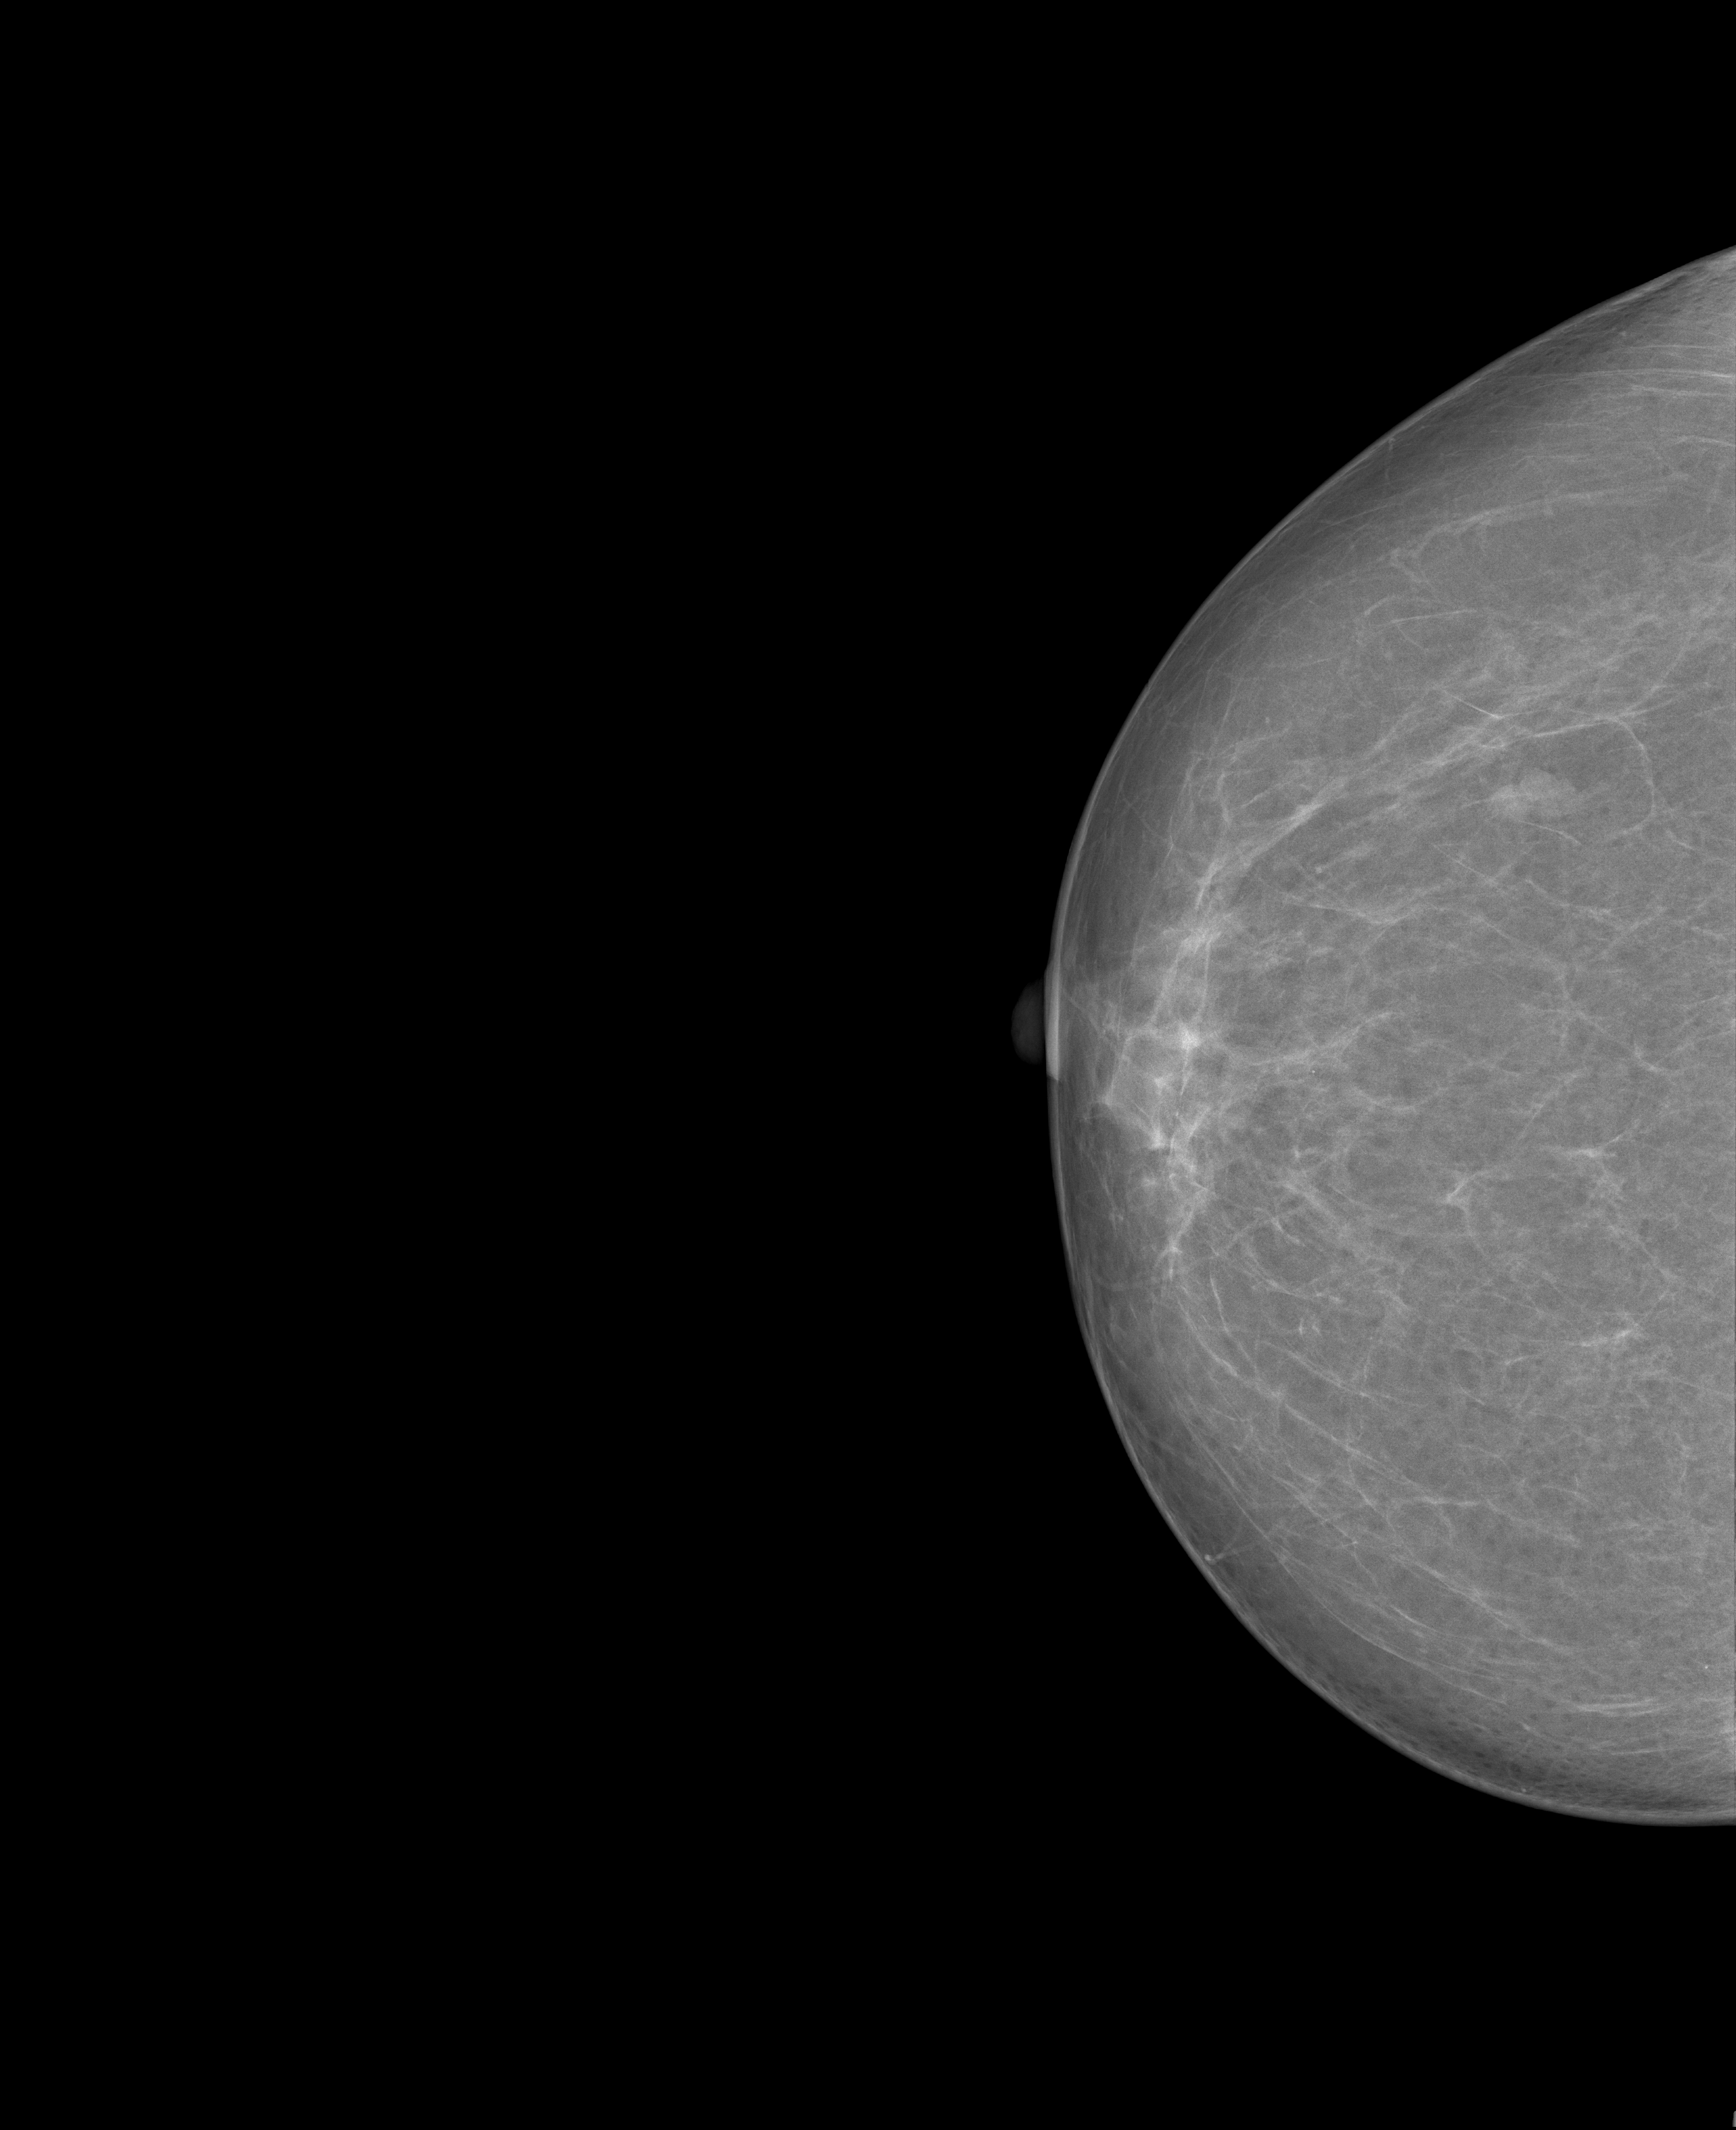
\includegraphics[height = 5cm]{plots/mammogram.png}
        \end{subfigure}
	\begin{subfigure}{4.2 cm}
		\centering
                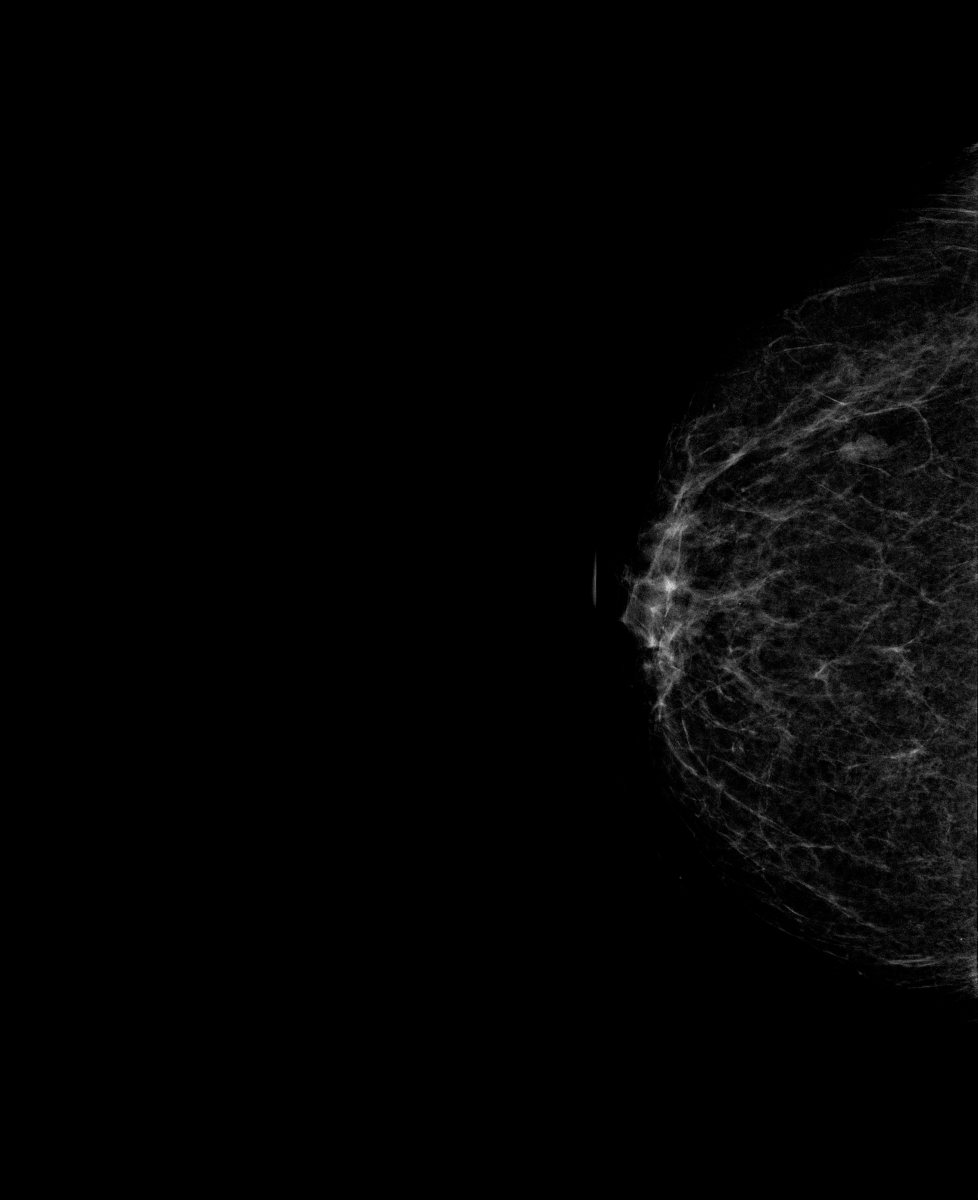
\includegraphics[height = 5cm]{plots/mammogram_enhanced.png}
        \end{subfigure}
	\begin{subfigure}{4.2 cm}
		\centering
                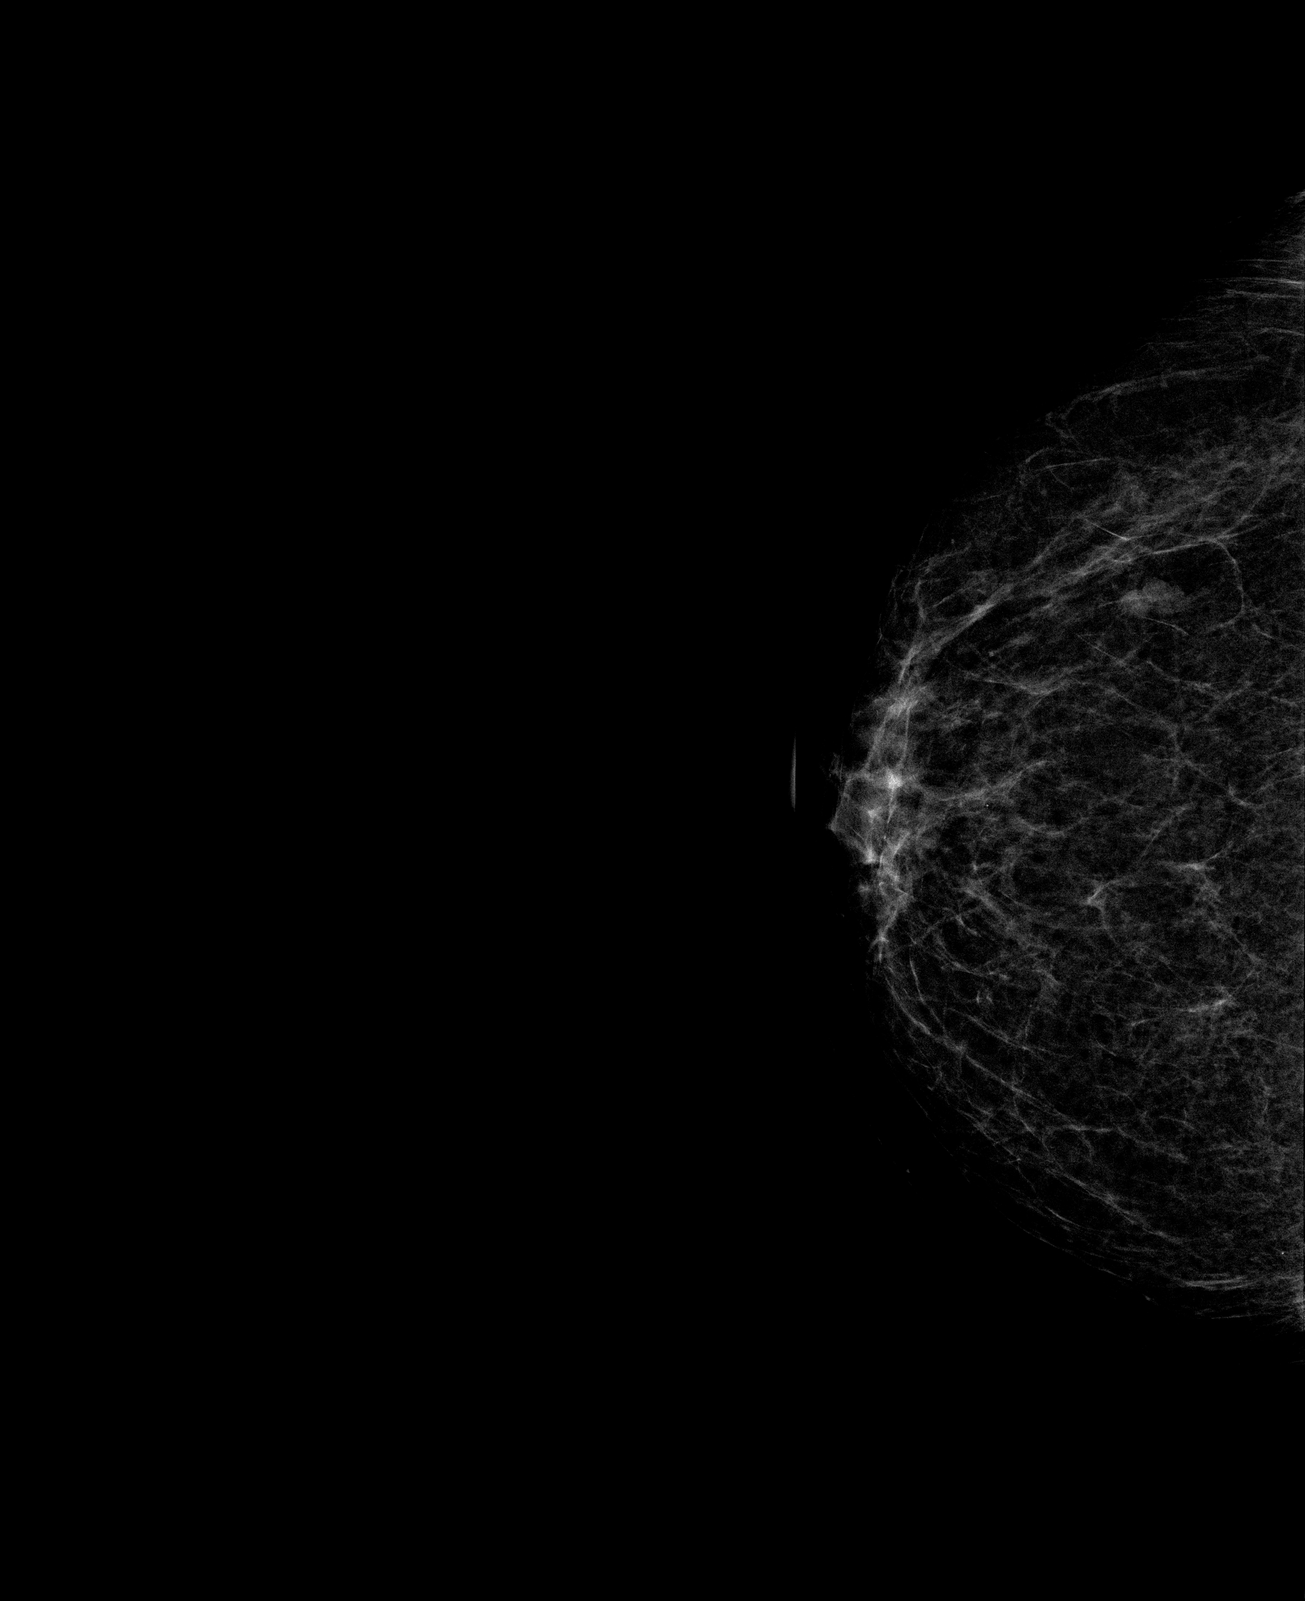
\includegraphics[height = 5cm]{plots/mammogram_resized.png}
        \end{subfigure}
	\begin{subfigure}{2.4 cm}
		\centering
                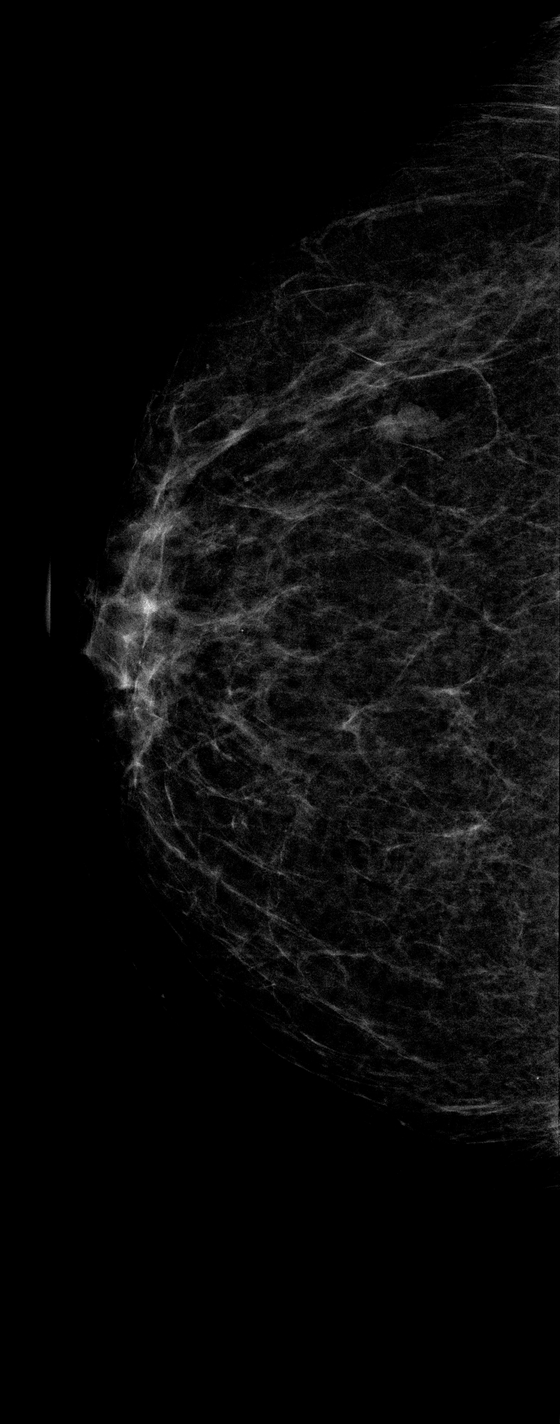
\includegraphics[height = 5cm]{plots/mammogram_v1.png}
        \end{subfigure}
	\\
	\begin{subfigure}{4.2 cm}
		\centering
                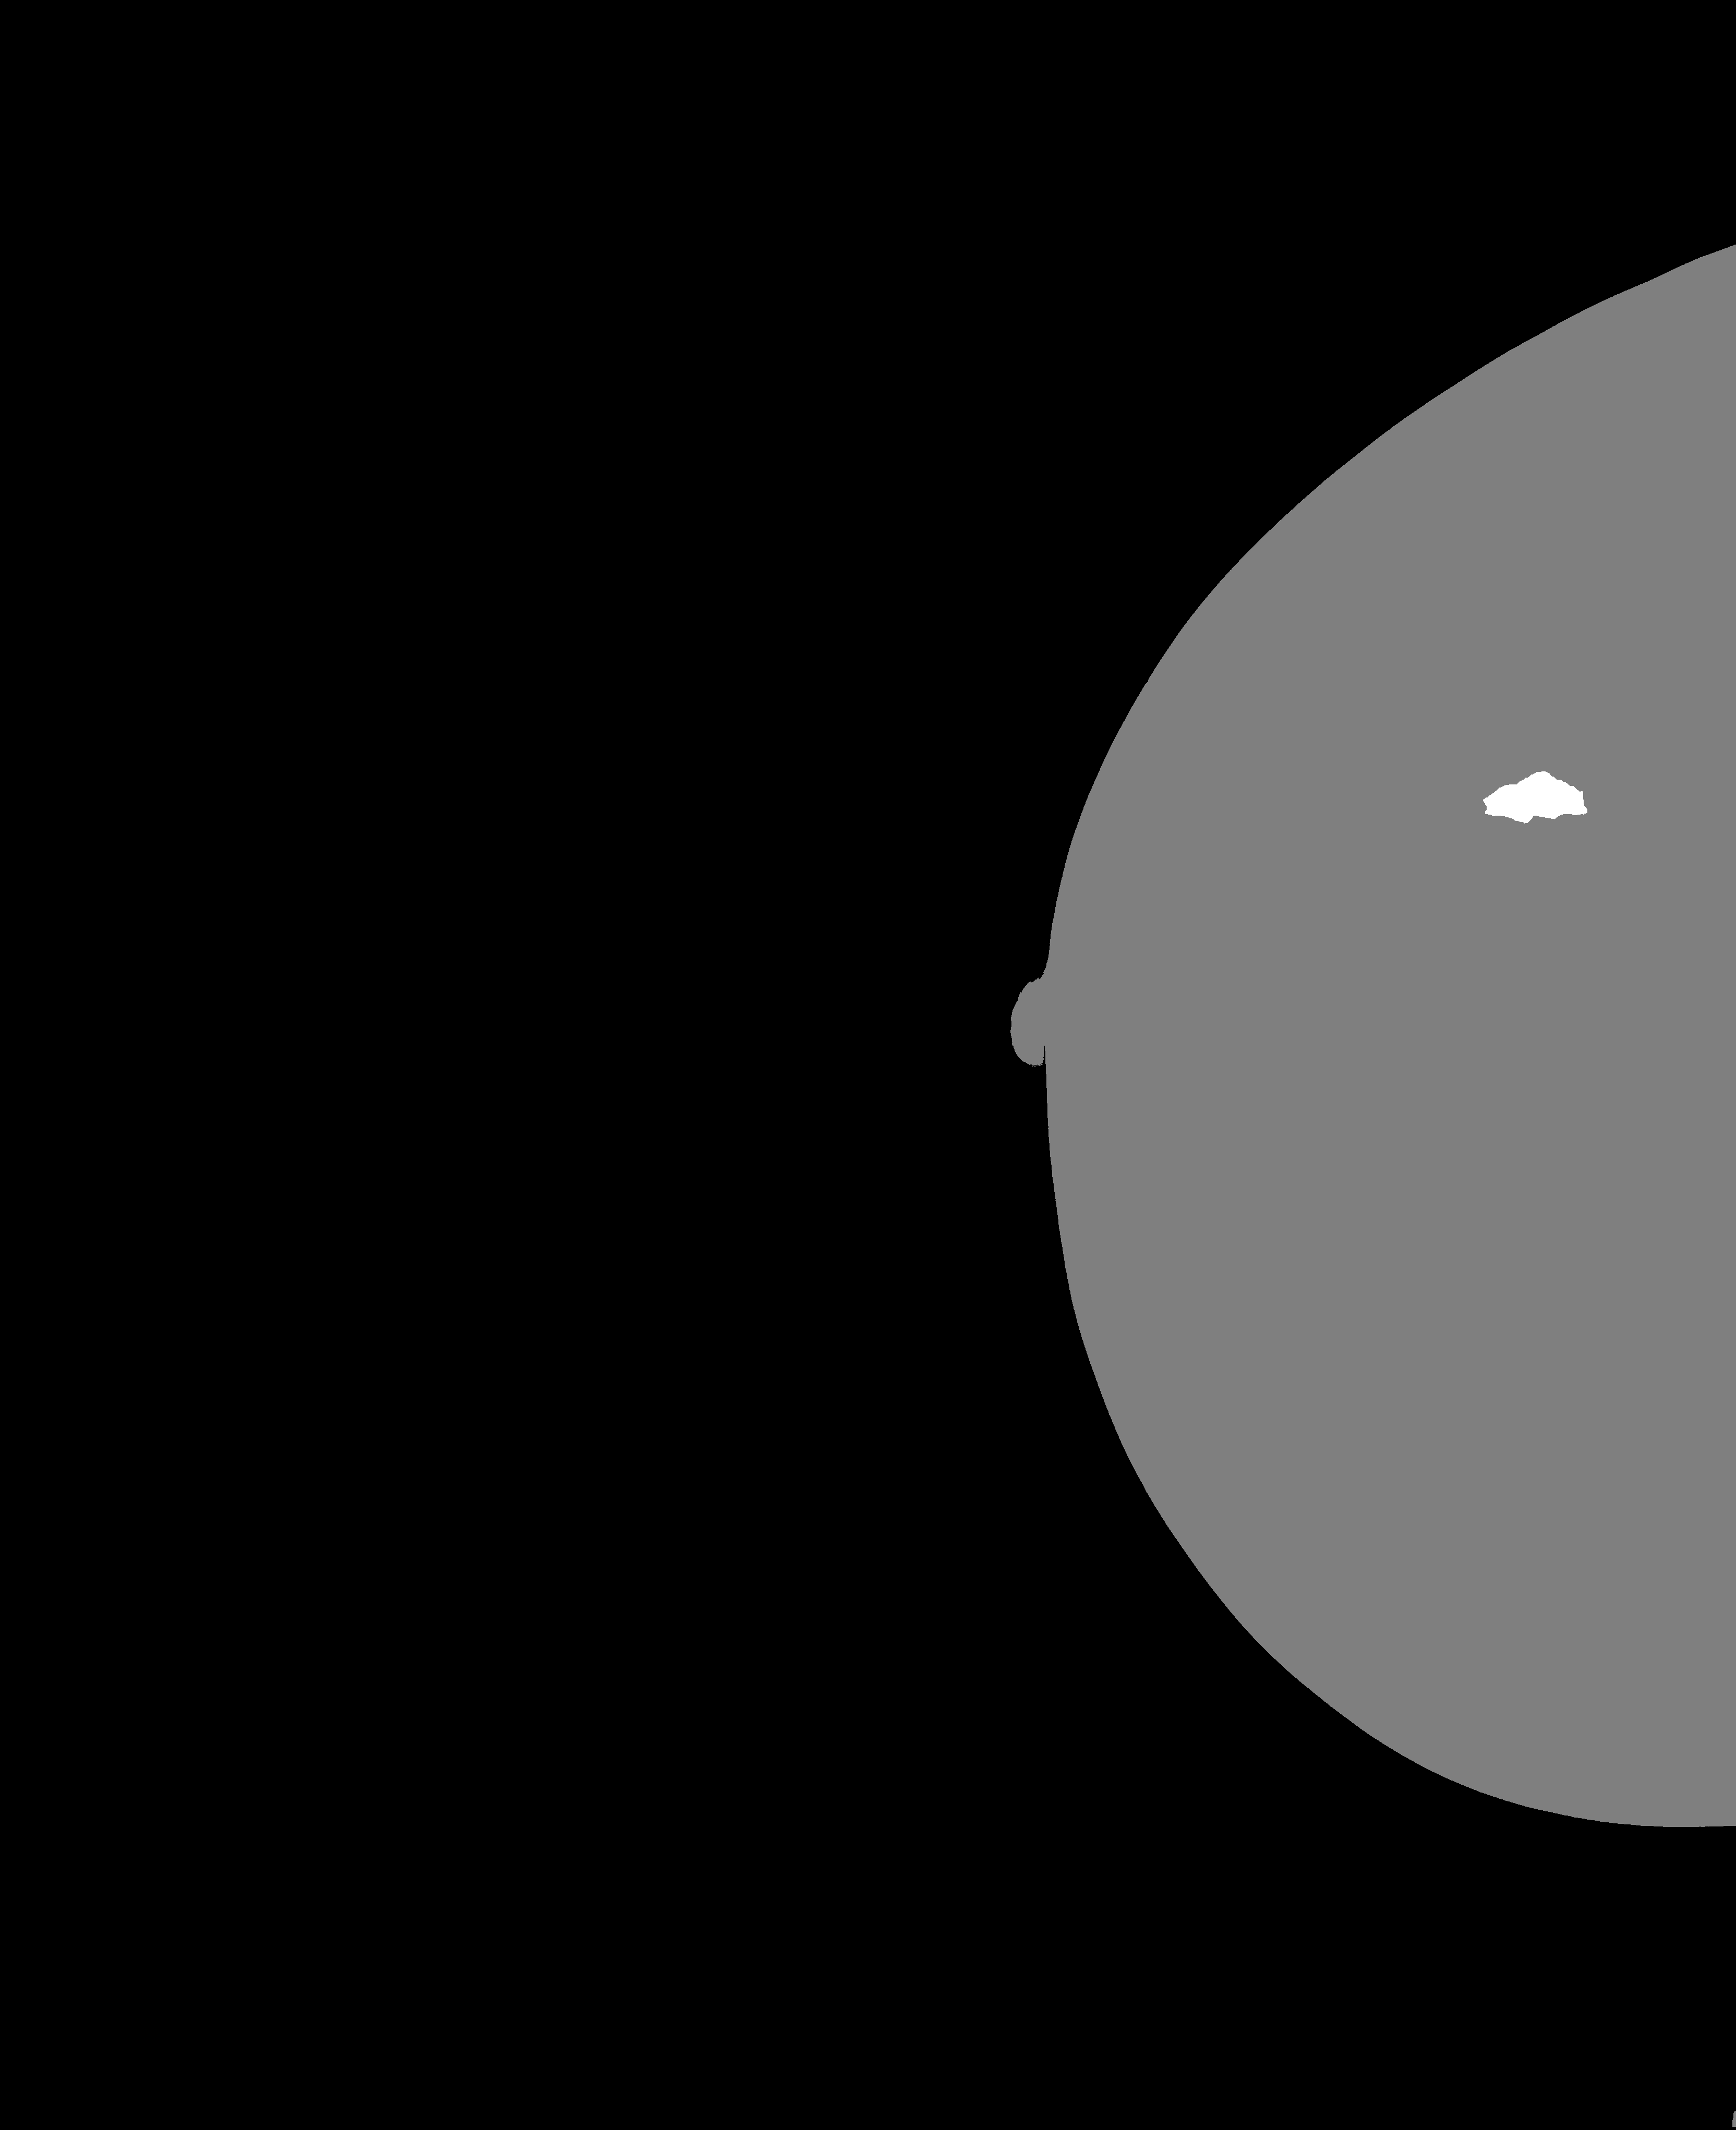
\includegraphics[height = 5cm]{plots/label.png}
		\caption{Original image}
		\label{subfig:Preprocessinga}
        \end{subfigure}
	\begin{subfigure}{4.2 cm}
		\centering
                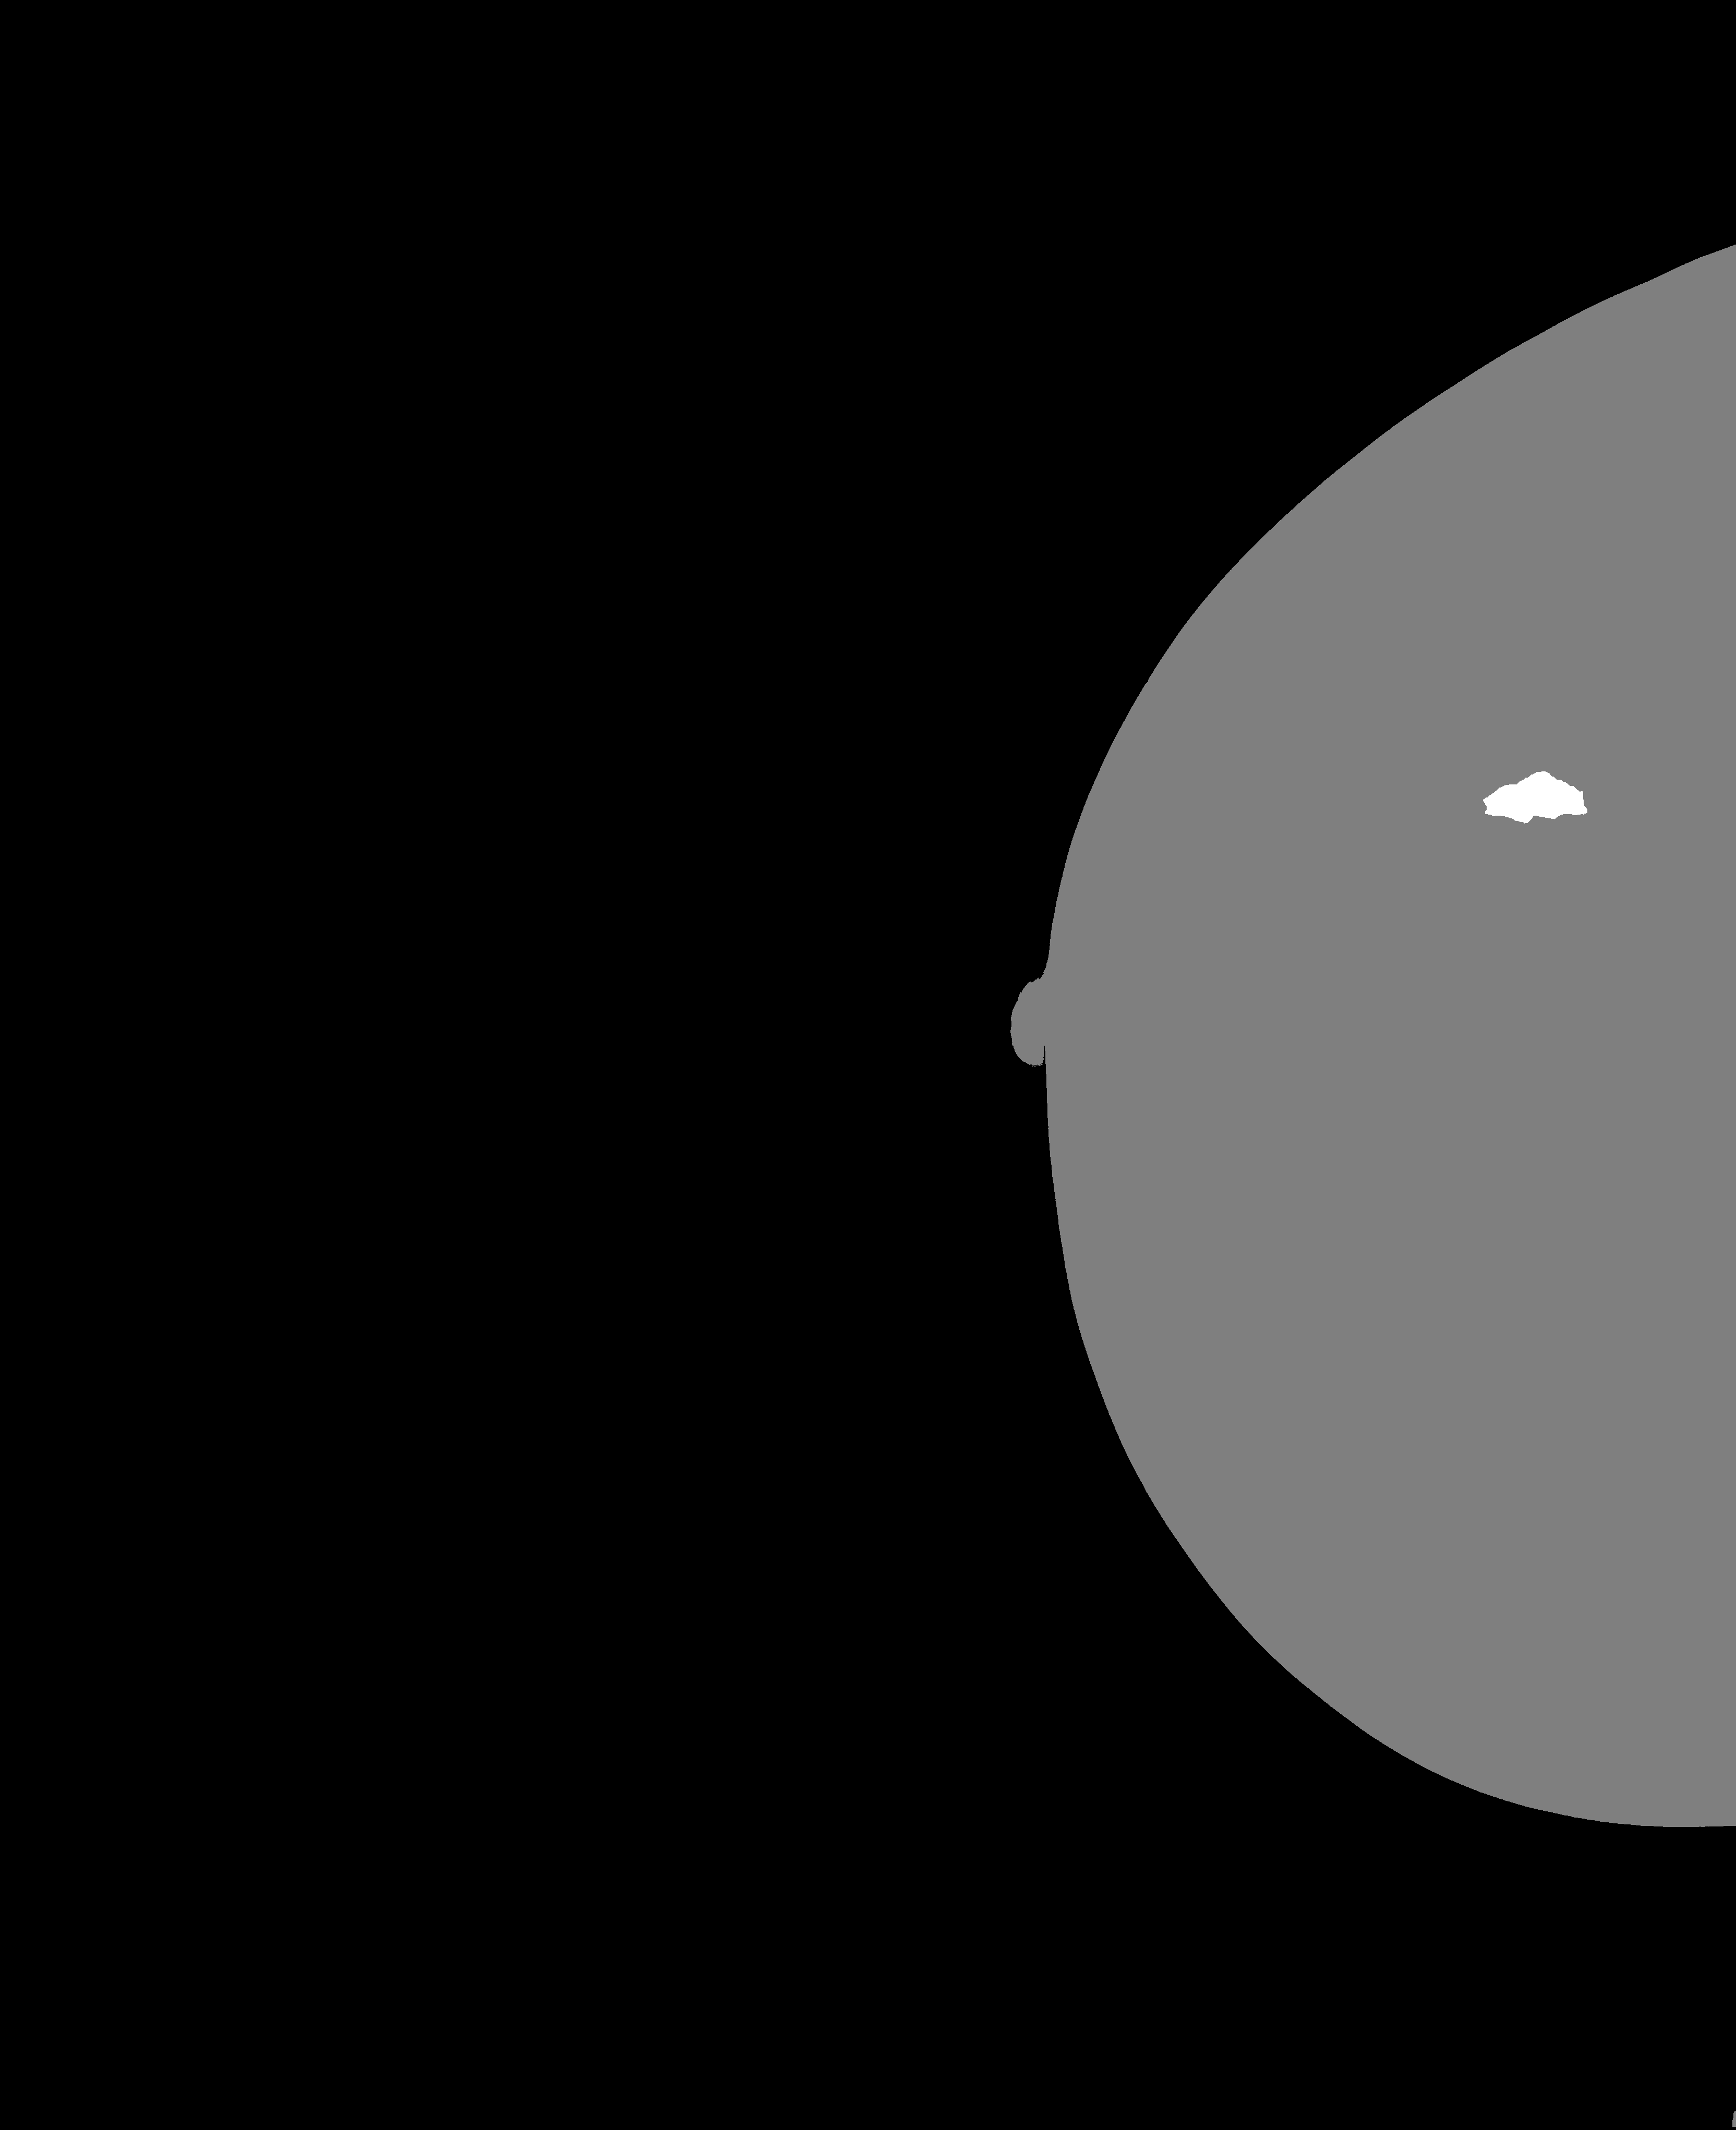
\includegraphics[height = 5cm]{plots/label_enhanced.png}
		\caption{Enhancement}
		\label{subfig:Preprocessingb}
        \end{subfigure}
	\begin{subfigure}{4.2 cm}
		\centering
                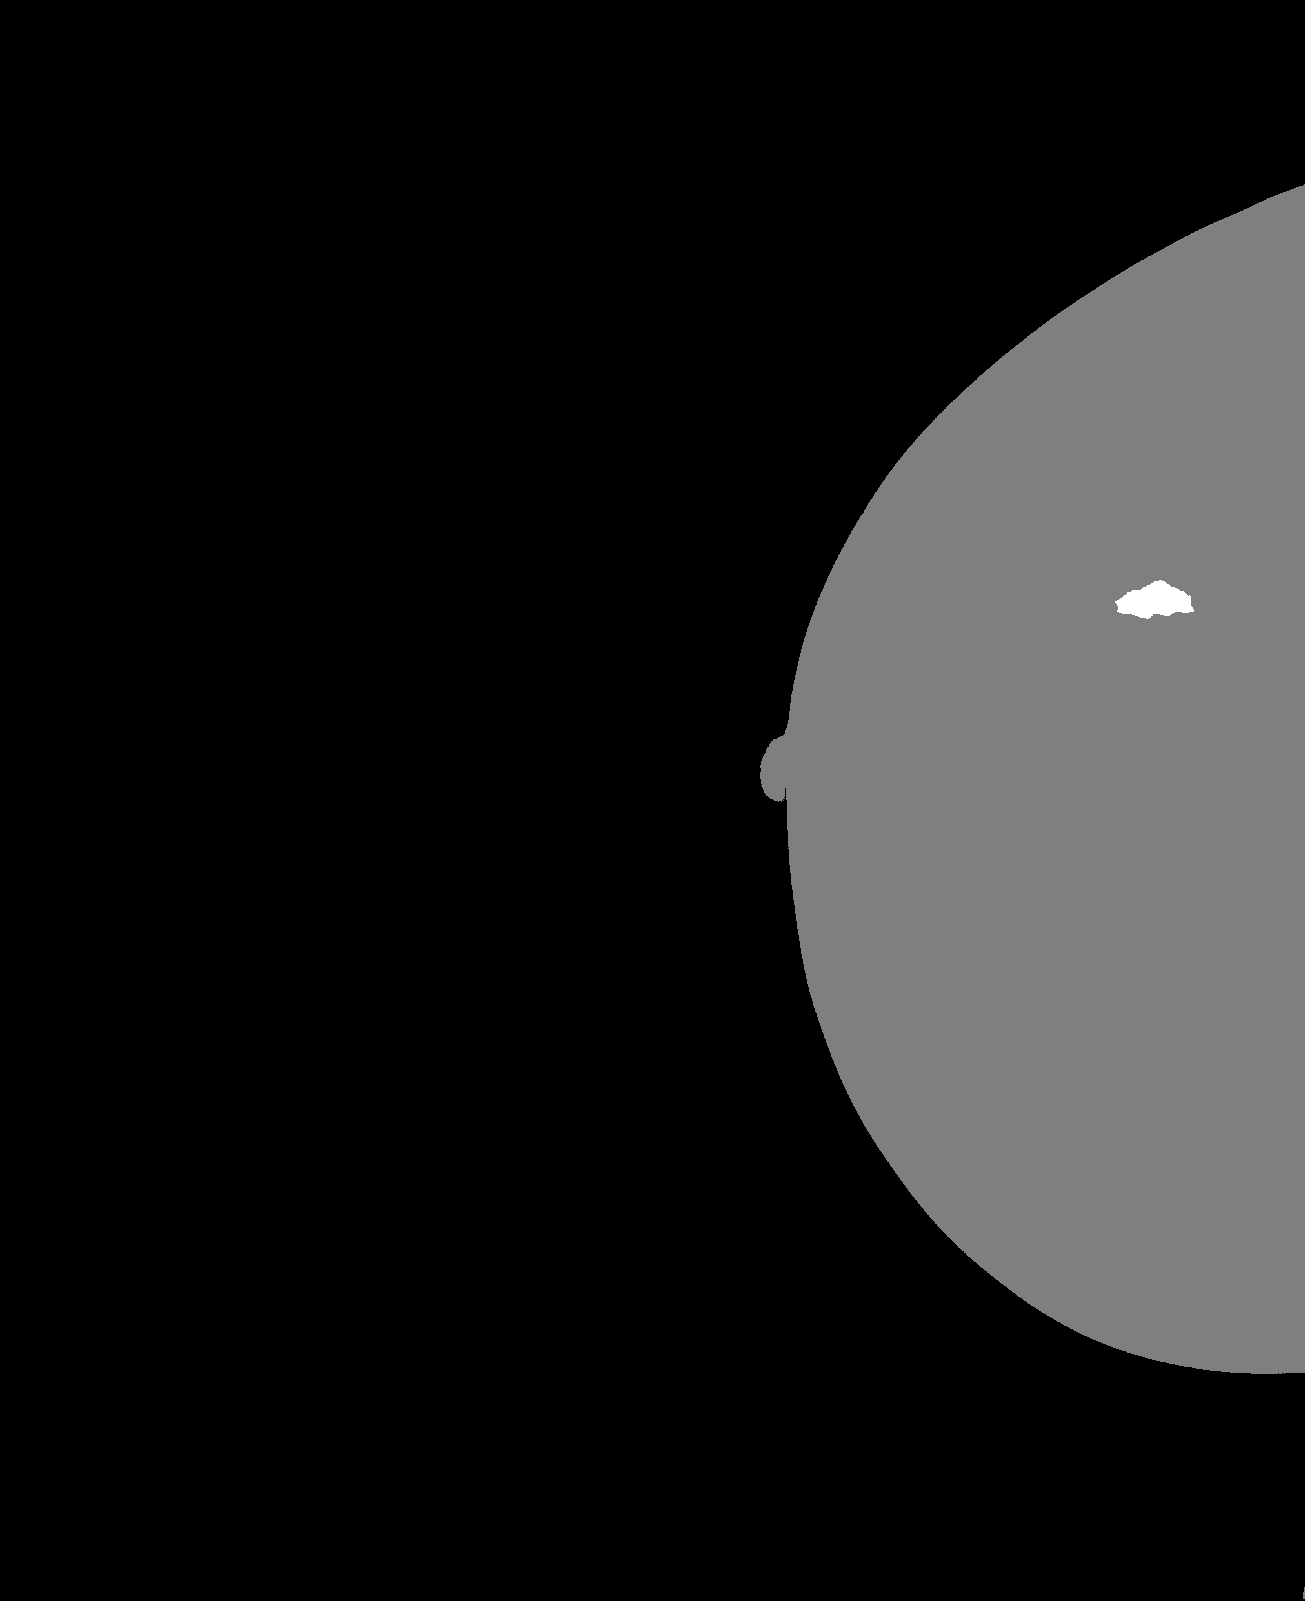
\includegraphics[height = 5cm]{plots/label_resized.png}
		\caption{Downsampling}
		\label{subfig:Preprocessingc}
        \end{subfigure}
	\begin{subfigure}{2.4 cm}
		\centering
		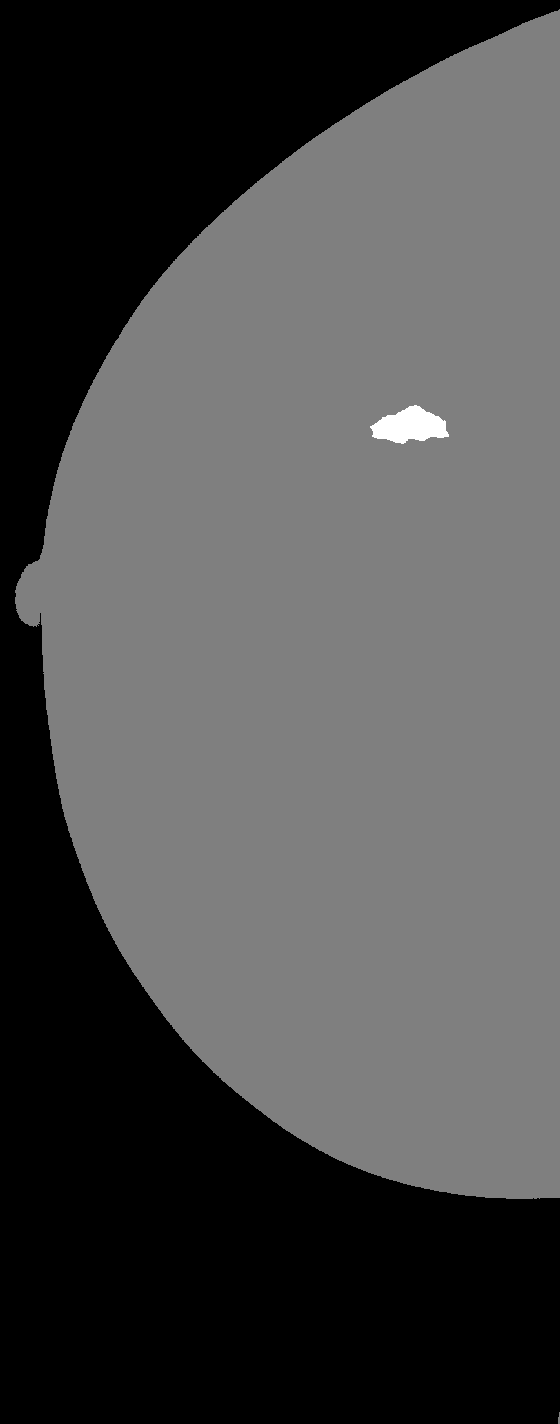
\includegraphics[height = 5cm]{plots/label_v1.png}
		\caption{Final image}
		\label{subfig:Preprocessingd}
        \end{subfigure}
	\caption[Preprocessing pipeline]{A mammogram (top) and its label (bottom) being preprocessed: (1) original images ($4084 \times 3328$), (2) background reduction plus contrast normalization, (3) downsampling and  (4) cropping to delete black spaces ($560 \times 1424$). Augmentation is not shown.}
	 \label{fig:Preprocessing}
% img_108_146_1_RCC.png
\end{figure}
	
\subsection{Data augmentation}
We mirror each image (mammograms and labels) and rotate the original and mirrored version at 0, 90, 180 and 270 degrees to increase our training and validation set by a factor of 8. 
%Mammograms and labels are mirrored and both the original and mirrored version rotated at 0, 90, 180 and 270 degrees to increase our training and validation set by a factor of 8. 
Images in the test set are not augmented.

This transformations are commonplace when training convolutional networks with small data sets. Because the test set is a proxy for real data, in principle, it should not be augmented.%In principle it is not neccesary to store the augmented images because they can be easily generated during training but if the disk space is not prohibitive explicitly storing them simplifies training.

%\subsection{Memory compromises} Hopefully not
% Cutting mammograms in 4 or 16 pieces for training would not be that bad, I would have to cut images surrounded with 48 pixels of surrounding regions so the netwrok also sees that and does not see black spaces, then to the output of the network i have to discard a surrounding region of 3 pixels all around to obtain the segmentation of my wanted image: this is exactkly as if training with the big entire image. This if i have no memory, or maybe if i want to change up a bit.

\subsection{Storage}
All augmented mammograms and their respective labels are stored as grayscale 8-bit images preserving their original names (plus a suffix) and folder organization.
% For training, a file enlisting the names of all the images is also generated.
The entire data set weights approximately 480 megabytes.
